% \subsection{Những thách thức đặt ra cho giải pháp tổng thể}
% \label{subsec:research_challenges}

% Từ những phân tích thực tiễn và tiền đề thực nghiệm nêu trên, luận văn đặt mục tiêu xây dựng một giải pháp AIOps hoàn chỉnh từ đầu đến cuối, tập trung giải quyết ba thách thức cốt lõi sau:

% \begin{enumerate}
%     \item \textbf{Hiệu chỉnh quyết định thẩm định theo nguồn gốc và nội dung bằng chứng:} Khi mở rộng đánh giá sang quy mô dữ liệu lớn với giao thức phân chia nghiêm ngặt theo từng đợt tiêm lỗi để chống rò rỉ dữ liệu, phân tích lỗi chuyên sâu cho thấy hiện tượng gia tăng đồng thời cả Recall lẫn tỷ lệ báo động giả (FPR) của truy xuất đồ thị vẫn tái diễn ($\Delta\mathrm{Recall} = +0,100$, $\Delta\mathrm{FPR} = +0,025$ trên tập tinh chỉnh)[cite: 5]. Tuy nhiên, nguyên nhân gốc rễ không phải do nhiễu từ các dịch vụ lân cận như giả định ban đầu, mà xuất phát từ \textit{thiên lệch xác nhận của LLM đối với các bằng chứng cục bộ sát thời điểm cảnh báo} (đặc biệt là các trace span có độ trễ nền vô hại)[cite: 5]. Do đó, thách thức đặt ra là thiết kế phương pháp thẩm định hiệu chỉnh (CTAV) kết hợp neo bằng chứng thực chất tại dịch vụ phát cảnh báo và ngưỡng tin cậy được hiệu chỉnh chặt chẽ, thay vì chỉ dựa vào các luật chặn cảm tính[cite: 5].
    
%     \item \textbf{Tự động hóa phân tích nguyên nhân gốc trên chuỗi cảnh báo đã thẩm định:} Một nền tảng vận hành hiệu quả không thể dừng lại ở việc phân loại từng cửa sổ cảnh báo rời rạc[cite: 4]. Hệ thống cần tích hợp một tác tử RCA tiếp nhận các cảnh báo đã được CTAV xác nhận, tự động gom cụm các cảnh báo xảy ra gần nhau thành từng sự cố thống nhất, thực hiện lan truyền ngược trên đồ thị gọi dịch vụ để xếp hạng dịch vụ nguyên nhân gốc và sinh báo cáo chẩn đoán JSON phục vụ kỹ sư SRE[cite: 4, 5].
    
%     \item \textbf{Kiểm soát ngân sách, kỷ luật đánh giá và trực quan hóa hệ thống:} Để đảm bảo tính khả thi trong môi trường sản xuất cũng như tính khách quan khoa học, toàn bộ chuỗi xử lý phải được đóng gói thành một nền tảng thống nhất có cơ chế lưu đệm (cache) định danh, tuân thủ giới hạn ngân sách gọi LLM, áp dụng quy trình đăng ký giả thuyết trước khi kiểm định độc lập trên tập kiểm thử, và cung cấp giao diện trực quan hóa theo dõi trạng thái vận hành từ lúc phát sinh cảnh báo đến khi xác định nguyên nhân gốc[cite: 1, 5].
% \end{enumerate}
\section{Giới thiệu đề tài}
\label{ch:mo-dau}
% \noindent \textit{Trong chương này, nhóm tác giả sẽ đưa ra tổng quan về đề tài, từ việc chỉ ra thực trạng quản lý tài sản công nghệ thông tin tại Việt Nam hiện nay, đến xác định rõ mục tiêu và phạm vi của đề tài mà nhóm tác giả đang thực hiện. Nhóm tác giả sẽ cung cấp một phân tích chi tiết về các yêu cầu của đề tài, làm sáng tỏ những khía cạnh quan trọng và đặc biệt trong quá trình nghiên cứu của nhóm tác giả. }
Trong các hệ thống phần mềm phân tán hiện đại xây dựng theo kiến trúc microservice, một sự cố cục bộ thường lan truyền nhanh qua nhiều services phụ thuộc và tạo ra hàng loạt cảnh báo đồng thời. Việc kết hợp các bộ Time-series Anomaly Detector với Mô hình Ngôn ngữ Lớn (LLM) mở ra khả năng tự động thẩm định cảnh báo và truy vết nguyên nhân gốc, song cũng đặt ra thách thức lớn về báo động xảy ra có là thật hay không, thiên lệch khi xác nhận và chi phí cho mỗi lần thẩm định. Đề tài này nghiên cứu và xây dựng một nền tảng AIOps, đi từ phát hiện bất thường dữ liệu metric, thẩm định cảnh báo có hiệu chỉnh theo bằng chứng đa phương thức, đến tự động hóa phân tích nguyên nhân gốc (RCA) và trực quan hóa vận hành. Chương 1 trình bày bối cảnh thực tiễn, những phát hiện thực nghiệm định hình bài toán, các mục tiêu, câu hỏi nghiên cứu, đóng góp chính, phạm vi thực hiện và bố cục tổng thể của đề tài.
\subsection{Bối cảnh và bài toán nghiên cứu}
\subsubsection{Vận hành AIOps trên hệ thống microservice và bài toán quá tải cảnh báo}
Kiến trúc microservice giúp các hệ thống đám mây đạt được tính linh hoạt, khả năng mở rộng theo chiều ngang và cô lập lỗi xảy ra tốt hơn so với kiến trúc \textit{monolithic} (nguyên khối). Tuy nhiên, khi hệ thống bị chia thành hàng chục đến hàng trăm dịch vụ độc lập, một yêu cầu từ người dùng có thể phải đi qua nhiều dịch vụ. Mỗi lần như vậy là một lần gọi qua mạng, nên luồng xử lý trở nên phức tạp hơn. Để giám sát trạng thái vận hành, các công cụ quan sát hiện đại thu thập liên tục ba nguồn dữ liệu telemetry chính: chuỗi thời gian chỉ số hiệu năng (\textit{metric}), nhật ký sự kiện bán cấu trúc (\textit{log}) và vết thực thi phân tán (\textit{trace}).

Trong thực tế vận hành, kỹ sư SRE thường dùng các công cụ tự động phát hiện bất thường trên dữ liệu metric (ví dụ thuật toán Isolation Forest~\cite{isof}) để giám sát hệ thống liên tục trên các khoảng thời gian gần nhất được cập nhật dần. Các mô hình này xử lý nhanh và tốn ít tài nguyên tính toán, nhưng vì chỉ dựa vào chuỗi số nên chúng không hiểu ngữ cảnh. Khi lưu lượng thay đổi theo chu kỳ hoặc có các tác vụ nền bình thường, chúng dễ báo động giả hàng loạt. Điều này gây \textbf{quá tải cảnh báo (alert fatigue)}~\cite{zhao2020alertstorm} và khiến đội vận hành phản ứng với sự cố chậm hơn.

Sự phát triển của các Mô hình Ngôn ngữ Lớn (LLM) giúp hệ thống có khả năng đọc hiểu và suy luận trên dữ liệu văn bản không đồng nhất như log và trace, từ đó phân biệt sự cố thật với nhiễu vận hành. Tuy vậy, khi đưa LLM vào quy trình giám sát và chẩn đoán sự cố, có ba nút thắt kỹ thuật chính:
\begin{enumerate}
    \item \textbf{Chi phí và độ trễ vận hành:} Nếu gọi LLM cho mọi khoảng dữ liệu giám sát thì chi phí API sẽ rất lớn, dễ chạm giới hạn số truy vấn và không đáp ứng được yêu cầu phản hồi nhanh của hệ thống giám sát liên tục.
    \item \textbf{Rủi ro ảo giác và thiên lệch xác nhận:} Khi thiếu ngữ cảnh vận hành phù hợp hoặc không bị buộc phải dựa trên bằng chứng cụ thể, LLM dễ suy diễn quá mức và đồng thuận theo gợi ý cảnh báo~\cite{sharma2024sycophancy}, coi những dao động vô hại là sự cố nghiêm trọng. Kết quả là báo động giả tăng lên thay vì giảm đi.
    \item \textbf{Khoảng trống từ thẩm định đến định vị nguyên nhân gốc:} Ngay cả khi từng cảnh báo riêng lẻ đã được lọc đúng, một sự cố lan rộng vẫn có thể tạo ra nhiều cảnh báo liên quan trên nhiều dịch vụ gọi nhau. Đội vận hành vẫn cần một cơ chế tự động để: gom các cảnh báo cùng thuộc một sự cố, truy ngược theo sơ đồ phụ thuộc giữa các dịch vụ để tìm đúng thành phần khởi phát sự cố (RCA), và tổng hợp thành báo cáo chẩn đoán có cấu trúc.
\end{enumerate}

\begin{figure}[H]
    \centering
     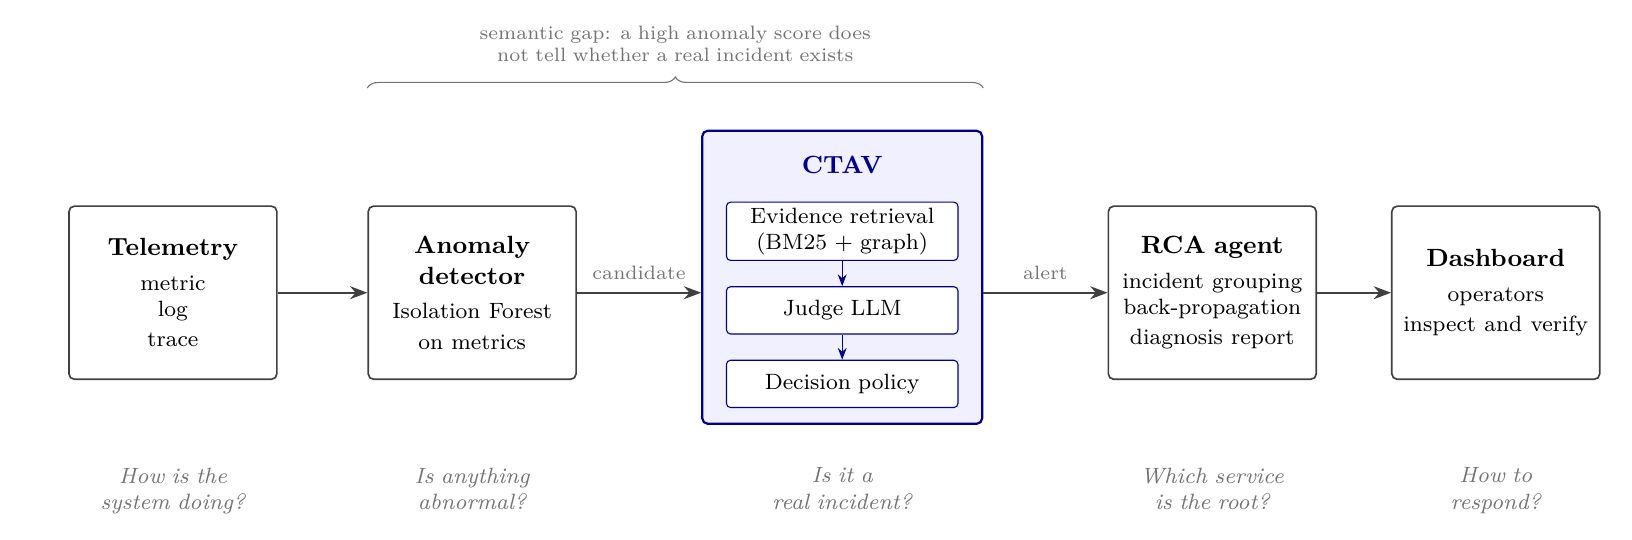
\includegraphics[width=0.88\textwidth]{Images/C1/figures/ch1/h1.1-system-overview.png}
    % \fbox{\parbox{0.85\textwidth}{\centering\vspace{1.2cm}\textit{Hình 1.1: Khoảng trống ngữ nghĩa của bộ phát hiện metric và quy trình từ thẩm định cảnh báo đến chẩn đoán nguyên nhân gốc]}}
    \vspace{0.5cm}
    \caption{Tổng quan hệ thống}
    \label{fig:ch1_alert_fatigue}
\end{figure}
\subsubsection{Khảo sát bước đầu về kiến trúc giám sát lai và đánh đổi ngữ cảnh đồ thị}  
Để giải quyết bài toán chi phí và khoảng trống ngữ nghĩa, hướng tiếp cận kiến trúc giám sát lai hai tầng được thiết lập: \textbf{tầng thứ nhất} sử dụng bộ phát hiện metric tốc độ cao để sàng lọc các cửa sổ đáng nghi thành danh sách cảnh báo ứng viên; \textbf{tầng thứ hai} kết hợp kỹ thuật RAG~\cite{lewis2020rag} trên dữ liệu log/trace với một LLM đóng vai trò bộ thẩm định (\textit{LLM-as-a-Judge})~\cite{zheng2023judging} xuất kết quả theo lược đồ JSON ràng buộc.

Trong quá trình khảo sát bước đầu tầng truy xuất bằng chứng trên bộ dữ liệu microservice Nezha~\cite{icaetm2026}, việc đối chiếu giữa truy xuất từ khóa truyền thống (BM25)~\cite{robertson2009bm25} và truy xuất mở rộng theo đồ thị gọi dịch vụ 2-hop (mở rộng \textit{2-hop} nghĩa là thu thập thêm bằng chứng log và trace từ các dịch vụ nằm cách dịch vụ phát cảnh báo tối đa hai bước liên kết trên đồ thị phụ thuộc (tính theo cả hai chiều gọi đến và được gọi)) đã bộc lộ một nghịch lý đáng chú ý trong thiết kế hệ thống giám sát lai (minh họa ở Hình~\ref{fig:ch1_alert_fatigue}):
\begin{itemize}
    \item \textbf{Lợi ích trong việc phát hiện sự cố lan truyền:} Nhiều sự cố hạ tầng (chẳng hạn độ trễ mạng) không sinh ra thông báo lỗi tường minh ngay tại dịch vụ phát cảnh báo, khiến truy xuất từ khóa cục bộ dễ bỏ sót do thiếu ngữ cảnh. Khi mở rộng phạm vi tìm kiếm sang các dịch vụ lân cận trên đồ thị phụ thuộc, hệ thống thu thập được chuỗi dấu vết liên đới giữa các dịch vụ gọi nhau, từ đó cải thiện rõ rệt khả năng nhận diện các sự cố lan truyền phức tạp.
    \item \textbf{Rủi ro bùng nổ báo động giả do thiếu hiệu chỉnh:} Trong trạng thái vận hành bình thường, truy xuất từ khóa thường trả về ngữ cảnh rỗng vì không có từ khóa lỗi, vô tình đóng vai trò như một lớp lọc nhiễu tự nhiên giúp bộ thẩm định LLM bác bỏ cảnh báo. Ngược lại, việc mở rộng ngữ cảnh theo đồ thị lại nạp thêm nhiều tín hiệu cảnh báo nền vô hại từ các dịch vụ xung quanh, dễ kích hoạt thiên lệch xác nhận ở LLM, làm gia tăng đột biến báo động giả và đẩy chi phí gọi API lên cao.
\end{itemize}
Phát hiện thực nghiệm này cho thấy truy xuất đồ thị và bộ thẩm định LLM không thể được thiết kế như hai mô-đun tách rời. Tuy nhiên, việc chỉ dừng lại ở nhận diện hiện tượng đánh đổi trên một tập mẫu cố định vẫn chưa giải quyết được toàn bộ bài toán vận hành thực tế.
\subsubsection{Những thách thức đặt ra cho giải pháp tổng thể}

Từ những phân tích thực tiễn và tiền đề thực nghiệm nêu trên, đề tài hướng tới xây dựng một giải pháp AIOps hoàn chỉnh từ đầu đến cuối, tập trung giải quyết ba thách thức cốt lõi sau:

\begin{enumerate}
    \item \textbf{Hiệu chỉnh quyết định thẩm định theo nguồn gốc và nội dung bằng chứng:} Khi mở rộng đánh giá sang quy mô dữ liệu lớn với quy trình phân chia chống rò rỉ dữ liệu theo từng đợt tiêm lỗi, phân tích chuyên sâu cho thấy hiện tượng gia tăng đồng thời cả khả năng phát hiện sự cố lẫn báo động giả của truy xuất đồ thị vẫn tái diễn. Tuy nhiên, nguyên nhân gốc rễ không phải do nhiễu từ các dịch vụ lân cận như giả định ban đầu, mà xuất phát từ \textit{thiên lệch xác nhận của LLM đối với các bằng chứng cục bộ sát thời điểm cảnh báo} (ngay cả khi đó chỉ là các dấu vết thực thi nền vô hại). Do đó, thách thức đặt ra là thiết kế phương pháp thẩm định hiệu chỉnh (CTAV) kết hợp cơ chế neo bằng chứng thực chất tại dịch vụ phát cảnh báo và ngưỡng tin cậy được hiệu chỉnh chặt chẽ, thay vì chỉ dựa vào các luật chặn cảm tính.
    
    \item \textbf{Tự động hóa phân tích nguyên nhân gốc trên chuỗi cảnh báo đã thẩm định:} Một nền tảng vận hành hiệu quả không thể dừng lại ở việc phân loại từng cửa sổ cảnh báo rời rạc. Hệ thống cần tích hợp một tác tử RCA tiếp nhận các cảnh báo đã được CTAV xác nhận, tự động gom cụm các cảnh báo liên quan thành từng sự cố thống nhất, thực hiện lan truyền ngược trên đồ thị gọi dịch vụ để xếp hạng dịch vụ khởi phát và sinh báo cáo chẩn đoán có cấu trúc phục vụ kỹ sư vận hành.
    
    \item \textbf{Kiểm soát ngân sách, kỷ luật đánh giá và trực quan hóa vận hành:} Để đảm bảo tính khả thi trong thực tế cũng như tính khách quan khoa học, toàn bộ chuỗi xử lý cần được đóng gói thành một nền tảng thống nhất. Hệ thống phải có cơ chế lưu đệm định danh nhằm tiết kiệm chi phí và tuân thủ giới hạn ngân sách gọi LLM, áp dụng kỷ luật kiểm định giả thuyết nghiêm ngặt trên tập dữ liệu độc lập, đồng thời cung cấp giao diện trực quan hóa xuyên suốt từ lúc phát sinh cảnh báo đến khi khoanh vùng nguyên nhân gốc.
\end{enumerate}

\subsection{Mục tiêu đề tài}
\subsubsection{Mục tiêu tổng quát}
Mục tiêu tổng quát của đề tài là nghiên cứu, đề xuất và kiểm chứng một giải pháp AIOps khép kín trên hệ thống microservice gồm ba khối liên kết chặt chẽ: phương pháp thẩm định cảnh báo hiệu chỉnh theo bằng chứng đa phương thức (\CTAV{}) nhằm giữ khả năng phát hiện sự cố lan truyền mà không làm tăng báo động giả trong cùng ngân sách gọi LLM; tác tử phân tích nguyên nhân gốc (RCA) gom các cảnh báo đã xác nhận, truy ngược đồ thị phụ thuộc để định vị dịch vụ khởi phát và sinh báo cáo chẩn đoán có cấu trúc; cùng nền tảng thực nghiệm thống nhất có bộ nhớ đệm định danh và giao diện trực quan hóa tái lập được.
\subsubsection{Mục tiêu cụ thể}
Để đạt các mục tiêu tổng quát trên, đề tài thực hiện năm mục tiêu cụ thể:
\begin{itemize}[label=--]
    \item \textbf{Xây dựng giao thức đánh giá chống rò rỉ và xác lập bài toán:}
    chia dữ liệu Nezha theo từng đợt tiêm lỗi, có vùng đệm thời gian giữa các split;
    trên giao thức đó, kiểm chứng rằng mở rộng ngữ cảnh theo topology làm tăng recall
    nhưng cũng làm tăng báo động giả so với truy xuất BM25.

    \item \textbf{Phân tích cơ chế báo động giả của judge LLM:}
    can thiệp có kiểm soát vào ngữ cảnh truy xuất (độ gần thời gian, loại bằng chứng,
    thứ tự trình bày) để xác định yếu tố khiến thẩm định xác nhận nhầm cửa sổ bình thường.

    \item \textbf{Đề xuất phương pháp CTAV:}
    kết hợp truy xuất hybrid BM25--topology, ngưỡng tin cậy cho quyết định của judge
    và cơ chế neo bằng chứng, chỉ chấp nhận cảnh báo khi chính service phát cảnh báo
    có tín hiệu bất thường.

    \item \textbf{Kiểm định theo giả thuyết đăng ký trước:}
    đánh giá một lần trên split \texttt{test} niêm phong bằng bootstrap CI~\cite{efron1993bootstrap} và McNemar~\cite{mcnemar1947note},
    gồm so sánh với các baseline, \textit{ablation} từng thành phần
    và hiệu quả theo ngân sách gọi LLM.

    \item \textbf{Xây dựng tác tử RCA và platform end-to-end:}
    gom cảnh báo đã thẩm định thành sự cố, lan truyền ngược trên đồ thị phụ thuộc
    để xếp hạng service gốc và sinh báo cáo chẩn đoán có cấu trúc; tích hợp toàn bộ
    pipeline với dashboard thành một platform chạy được và tái lập được từ \textit{cache}.
\end{itemize}
\subsection{Đối tượng và phạm vi nghiên cứu}
\label{subsec:scope}

\subsubsection{Đối tượng nghiên cứu}
\label{subsubsec:research_objects}

Đề tài tập trung vào ba đối tượng trong chuỗi giám sát và chẩn đoán sự cố tự động trên microservice:
\begin{itemize}[label=--]
    \item \textbf{Dữ liệu quan sát đa phương thức và đồ thị phụ thuộc:} cửa sổ metric, log, trace và đồ thị gọi dịch vụ dựng từ trace.
    \item \textbf{Phương pháp thẩm định cảnh báo \CTAV{}:} truy xuất lai theo từ vựng--topology, bộ thẩm định LLM có cấu trúc và chính sách neo bằng chứng tại dịch vụ phát cảnh báo.
    \item \textbf{Tác tử RCA và nền tảng thực nghiệm:} gom cụm sự cố, lan truyền ngược xếp hạng dịch vụ gốc, báo cáo chẩn đoán JSON và dashboard trực quan hóa.
\end{itemize}

\subsubsection{Phạm vi nghiên cứu}
\label{subsubsec:research_scope}

Phạm vi của đề tài được giới hạn ở ba khía cạnh:
\begin{itemize}[label=--]
    \item \textbf{Dữ liệu và môi trường:} một bộ dữ liệu công khai là Nezha~\cite{nezha}, thu từ hai hệ microservice
mẫu (OnlineBoutique, TrainTicket) với các loại lỗi tiêm có chủ đích (độ trễ mạng, tranh chấp và
tiêu thụ CPU, ngoại lệ, giá trị trả về sai). Dữ liệu được chia theo từng đợt tiêm lỗi để chống
rò rỉ; chỉ số chính tính trên các cửa sổ có telemetry. Hệ thống chạy bằng cách phát lại dữ liệu
và đọc lại từ \textit{cache}, không triển khai trên hạ tầng production và chưa kiểm chứng trên
bộ dữ liệu khác.

    \item \textbf{Mô hình:} bộ phát hiện bất thường cố định là Isolation Forest. Judge và bộ tóm tắt
    sự cố dùng một LLM duy nhất qua API (\texttt{gemini-2.5-flash}~\cite{google2026gemini}, temperature 0); đề tài không
    fine-tuning và không dùng LLM cục bộ.

    \item \textbf{Đánh giá:} chất lượng thẩm định cảnh báo (Precision, Recall, F1, FPR), định vị
    dịch vụ gốc (Hit@$k$, tỷ lệ giảm cảnh báo), chi phí gọi LLM theo ngân sách, và độ ổn định
    của judge khi gọi lặp lại. Mọi so sánh giữa các phương pháp đều kèm khoảng tin cậy bootstrap
    và kiểm định McNemar.
\end{itemize}

\subsection{Ý nghĩa của đề tài}
\label{subsec:significance}

\subsubsection{Ý nghĩa thực tiễn}
\label{subsubsec:practical_significance}

Trên hệ thống microservice, bộ phát hiện bất thường dựa trên metric sinh ra nhiều cảnh báo, phần lớn không ứng với sự cố thật. Mỗi cảnh báo sai lấy đi thời gian của đội vận hành và làm giảm niềm tin vào hệ thống giám sát. Đề tài đặt một judge LLM sau bộ phát hiện để đọc bằng chứng log và trace trước khi xác nhận cảnh báo. Kết quả thực nghiệm cho thấy cung cấp thêm ngữ cảnh không tự động làm quyết định tốt hơn: ngữ cảnh theo topology giúp bắt thêm sự cố nhưng cũng kéo theo báo động giả. Vì vậy, khi triển khai cần một chính sách quyết định kiểm soát được nguồn gốc của bằng chứng, chứ không chỉ một bộ truy xuất tốt hơn.

Đề tài đo hiệu quả theo số lần gọi LLM, nhờ đó đội vận hành có thể ước lượng chi phí trước khi
triển khai. Tác tử RCA nối tiếp quá trình này: gom các cảnh báo đã thẩm định thành sự cố, chỉ ra dịch vụ gốc và sinh báo cáo chẩn đoán có cấu trúc, rút ngắn bước chẩn đoán thủ công. Toàn bộ chuỗi xử lý chạy trên một platform tái lập được từ \textit{cache}, có thể dùng làm môi trường thử chính sách thẩm định trước khi áp dụng lên hệ thống thật. Các kết quả này thu được trên dữ liệu phát lại của Nezha; áp dụng cho hệ thống production cần được kiểm chứng thêm.

\subsubsection{Ý nghĩa khoa học}
\label{subsubsec:scientific_significance}

Về mặt khoa học, đề tài làm rõ vì sao ngữ cảnh topology làm tăng báo động giả của judge LLM.
Giả thuyết ban đầu cho rằng bằng chứng từ các dịch vụ lân cận gây nhiễu, nhưng thực nghiệm có kiểm soát không ủng hộ giả thuyết này. Nguyên nhân phù hợp hơn là thiên lệch xác nhận: judge dễ xác nhận cảnh báo khi gặp bằng chứng cục bộ nằm sát thời điểm cảnh báo, nhất là bằng chứng từ trace. Phát hiện này chuyển trọng tâm từ câu hỏi ``truy xuất gì'' sang câu hỏi ``quyết định thế nào với bằng chứng đã truy xuất'', và là cơ sở thiết kế phương pháp CTAV.

Đề tài cũng đóng góp về phương pháp luận cho việc đánh giá LLM trong AIOps. Dữ liệu được chia theo từng đợt tiêm lỗi để chống rò rỉ; giả thuyết và tiêu chí bác bỏ được đăng ký trước khi tiếp cận tập kiểm thử; mọi so sánh đều kèm khoảng tin cậy bootstrap và kiểm định McNemar thay vì một điểm số đơn lẻ. Các thiết kế không đạt kỳ vọng, như ngưỡng riêng theo nguồn bằng chứng, định tuyến hai tầng và cơ chế cứu cảnh báo, được báo cáo cùng bằng chứng loại bỏ. Những kết quả âm này giúp các nghiên cứu sau tránh lặp lại các thiết kế đã được kiểm chứng là không hiệu quả.
% \subsection{Cấu trúc báo cáo}
% % \subsection{Cấu trúc báo cáo}
% \noindent Báo cáo \textbf{Thực tập 1} này gồm 7 chương, với các nội dung chính được trình
% bày trong bảng sau:
% \begin{longtable}{|>{\centering\arraybackslash}m{2cm}|>{\centering\arraybackslash}m{10cm}|}
%     \caption{Cấu trúc báo cáo Đồ án Chuyên ngành} \\
%     \hline
%     \textbf{Chương} & \textbf{Nội dung} \\
%     \hline
%     \endfirsthead

%     \hline
%     \textbf{Chương} & \textbf{Nội dung} \\
%     \hline
%     \endhead 
%     1 & Giới thiệu tổng quan đề tài\\  
%     \hline 
%     2 & Kiến thức và công nghệ nền tảng \\  
%     \hline 
%     3 & Các công trình liên quan \\  
%     \hline 

%     4 & Hệ thống đề xuất\\  
%     \hline 

%     5 & Phân tích và thiết kế \\  
%     \hline 
%     6 & Hiện thực và kiểm thử \\  
%     \hline 
%     7 & Triển khai hệ thống\\  
%     \hline 
%     8 & Đánh giá hệ thống \\  
%     \hline 
%     9 & Tổng kết \\  
%     \hline 
    
    
% \end{longtable}